%   ------------------------------------------------------------------------
\FloatBarrier
\subsection{Geração da animação de caminhada}
\label{s.gemini.animacaoAndar}

Como comentado anteriormente, a geração de vídeo era limitada a três animações por dia. Esse fator fez com que, antes mesmo de ter o sprite final em side view do personagem, fossem realizados testes para produzir o movimento de caminhada. Só era possível anexar uma única imagem e o prompt tinha que ser reescrito novamente a cada resultado gerado. Todos os vídeos produzidos possuem som, porém o foco da análise foi especificamente no conteúdo visual produzido, sem levar em conta o material sonoro.


Durante os testes iniciais (Figuras \ref{fig:geminiProAndar1} e \ref{fig:geminiProAndar2} no Apêndice \ref{ap.telasIA}), foi utilizado o sprite do personagem em front view como imagem a ser transformada em vídeo. Os resultados\footnote{\url{https://drive.google.com/drive/folders/1rbBwuVsgvShD8JoruLJN_poLJRwVSOcO?usp=sharing}} gerados mantiveram em grande parte a pixel art, criaram precisamente o movimento de caminhada e formaram o sprite em side view consistente com o estilo, porém apresentando incongruências em relação a características físicas específicas e aos tons de cores (Figura \ref{fig:GeminiProAndarComparaSprite}). Um detalhe interessante de ser ressaltado foi que, diferente das outras ferramentas de vídeo, a animação não deformou completamente a pixel art, como pode ser visto na Figura \ref{fig:geminiProAndarQuadroPixelCoerente}. Apesar da alta qualidade, a inconsistência chamativa na aparência fez com que esses vídeos não fossem considerados satisfatórios para a animação no jogo.

\begin{figure}[htbp]
    \centering
    \caption{\small Comparação do sprite em front view com os sprites em side view das animações geradas no Gemini Pro}
    \label{fig:GeminiProAndarComparaSprite}
    \begin{subfigure}{0.32\linewidth}
        \centering
        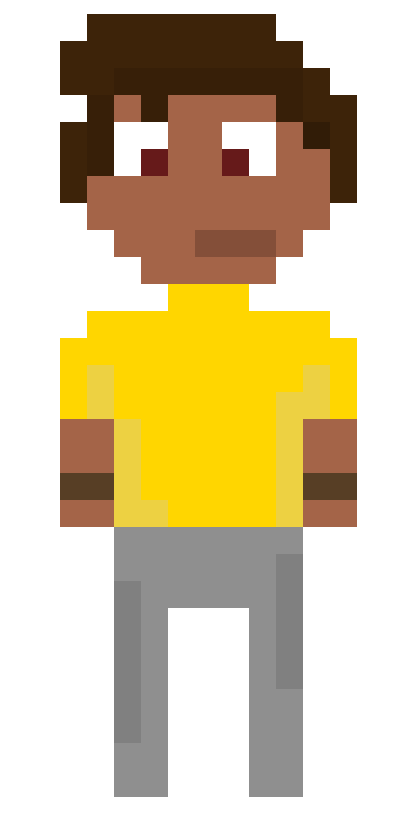
\includegraphics[width=0.7\linewidth]{figs/sprites/Pablo.PNG}
        \caption{\small Sprite do Pablo em front view, sem sapato visível}
        \label{fig:GeminiProAndaPablo}
    \end{subfigure}
    \begin{subfigure}{0.32\linewidth}
        \centering
        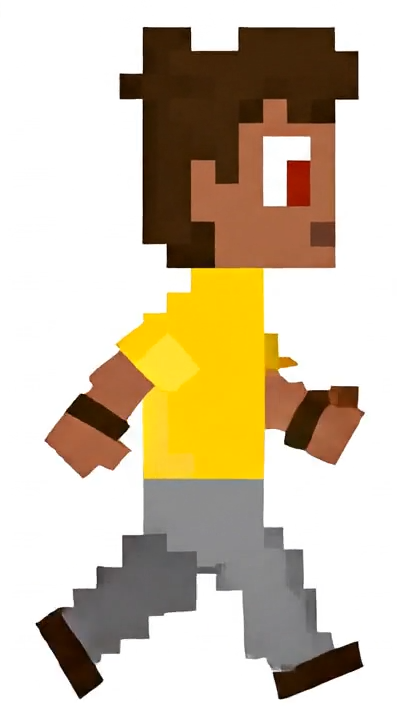
\includegraphics[width=0.7\linewidth]{figs/geminiPro/chat3/sprite1.PNG}
        \caption{\small Sprite com adição de sapatos pretos e olhos de cor e tamanho diferente da referência}
        \label{fig:GeminiProAndarComparaSprite1}
    \end{subfigure}
    \begin{subfigure}{0.32\linewidth}
        \centering
        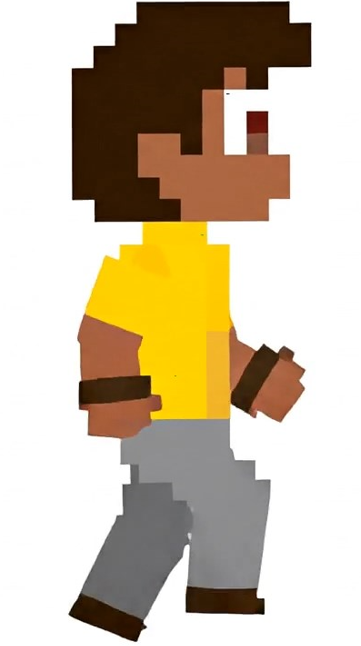
\includegraphics[width=0.7\linewidth]{figs/geminiPro/chat3/sprite2.PNG}
        \caption{\small Sprite com olho maior que a referência e pupila de dois tons de cores}
        \label{fig:GeminiProAndarComparaSprite2}
    \end{subfigure}

    \legend{\small Fonte: Elaborada pela autora, utilizando a ferramenta Gemini Pro.}
\end{figure}

\begin{figure}[htbp]
    \centering
    \caption{\small Quadro da animação de caminhada gerada no Gemini Pro, circulada em vermelho a diagonal incoerente com pixel art e circulada em azul a diagonal pixelizada de forma coerente}
    \label{fig:geminiProAndarQuadroPixelCoerente}
    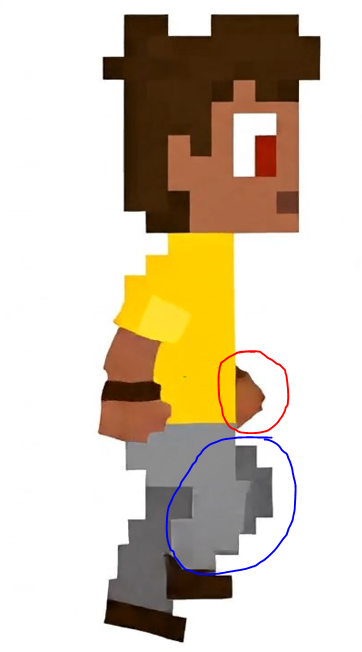
\includegraphics[width=0.3\linewidth]{figs/geminiPro/chat3/animacaoPixelArt.PNG}
    \legend{\small Fonte: Elaborada pela autora, utilizando a ferramenta Gemini Pro.}
\end{figure}

No teste seguinte (Figura \ref{fig:geminiProAndar3} no Apêndice \ref{ap.telasIA}), foi anexado o melhor sprite em side view que havia até aquele momento (Figura \ref{geminiProSideCompararMelhor2}), fazendo com que não se precisasse gerar um sprite em side view junto com o vídeo, sendo necessário produzir apenas a animação. O resultado\footnote{\url{https://drive.google.com/file/d/1dQZF4InImDsFU4jw68rXUGffW1hfGMWA/view?usp=sharing}} foi extremamente consistente com a referência e apresentou o movimento correto de andar. A animação deforma a pixel art de modo a formar diagonais incoerentes, porém essa falha não foi muito chamativa. Apesar disso, o vídeo possuía um erro grave que tornava o mesmo inadequado para uso: durante a animação, quando o braço se move, é revelado um buraco nas costas. Isso pode ser visto na Figura \ref{fig:GeminiProAndarFuroCostas}. 
\begin{figure}[htbp]
    \centering
    \caption{\small Comparação do sprite em side view de referência com o sprite da animação gerada no Gemini Pro}
    \label{fig:GeminiProAndarFuroCostas}
    \begin{subfigure}{0.45\linewidth}
        \centering
        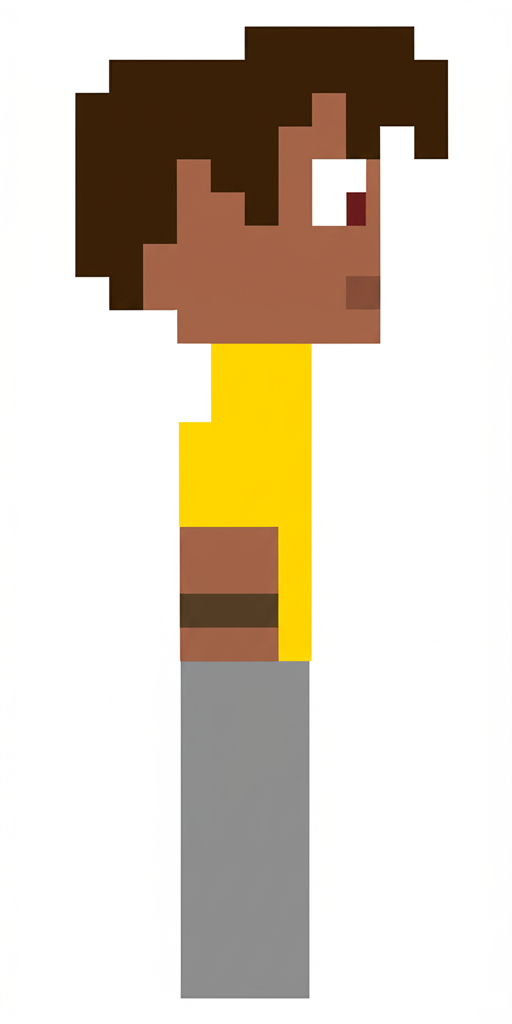
\includegraphics[width=0.3\linewidth]{figs/geminiPro/chat2/res1_tela1.png}
        \caption{\small Sprite do Pablo em side view}
        \label{fig:GeminiProAndarFuroCostasReferencia}
    \end{subfigure}
    \begin{subfigure}{0.45\linewidth}
        \centering
        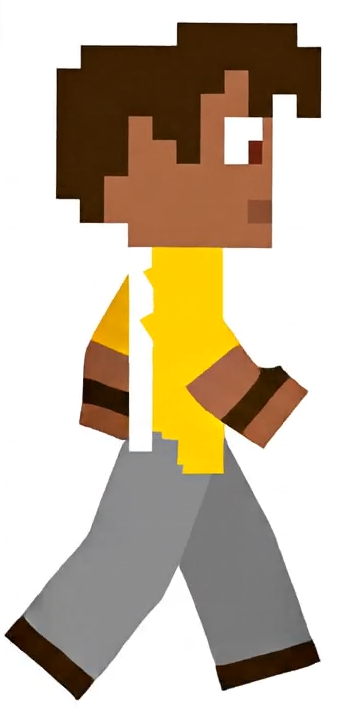
\includegraphics[width=0.3\linewidth]{figs/geminiPro/chat3/sprite3.PNG}
        \caption{\small Quadro da animação de caminhada revelando o vão nas costas}
        \label{fig:GeminiProAndarFuroCostasResultado}
    \end{subfigure}

    \legend{\small Fonte: Elaborada pela autora, utilizando a ferramenta Gemini Pro.}
\end{figure}

Analisando a imagem de referência, foi teorizado que a maneira em que o sprite estava desenhado foi responsável por fazer com que a IA entendesse que a linha do corpo acabava antes (Figura \ref{fig:geminiProAndarLinhaCorpo}), o que ficava desconectado da perna e criava o vão. 

\begin{figure}[htbp]
    \centering
    \caption{\small Linha preta representando possível interpretação do modelo de IA sobre onde o torso terminava}
    \label{fig:geminiProAndarLinhaCorpo}
    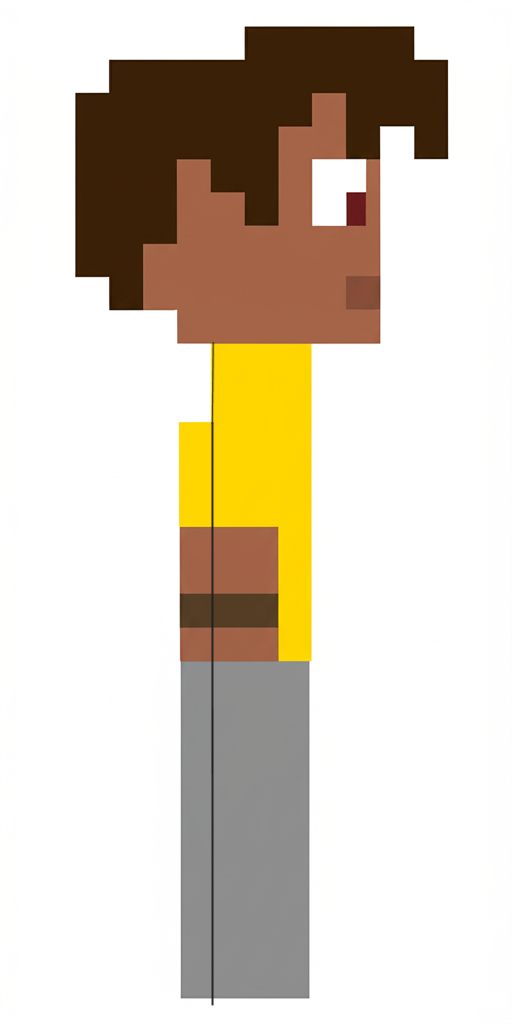
\includegraphics[width=0.3\linewidth]{figs/geminiPro/chat3/linhaCorpo.png}
    \legend{\small Fonte: Elaborada pela autora, utilizando a ferramenta Gemini Pro.}
\end{figure}

Para evitar essa falha, o sprite apresentado abaixo na Figura \ref{fig:GeminiProAndarSide1} foi usado como referência no teste posterior (Figura \ref{fig:geminiProAndar4} no Apêndice \ref{ap.telasIA}). O resultado\footnote{\url{https://drive.google.com/file/d/1Bi-5QSThXMqe6zONrDluai8ukYTAYkVj/view?usp=sharing}} gerado foi satisfatório, apresentando alta consistência e precisão. Apesar disso, o vídeo adicionou sapatos pretos no personagem e apresentou distorções na região dos joelhos e das mãos (Figura \ref{fig:GeminiProAndarDeformacao}, além da animação deformar a pixel art fazendo-a perder a coerência. 

\begin{figure}[htbp]
    \centering
    \begin{minipage}{0.45\textwidth}
        \centering
        \caption{\small Sprite em side view usado como referência na geração da animação no Gemini Pro}
        \label{fig:GeminiProAndarSide1}
        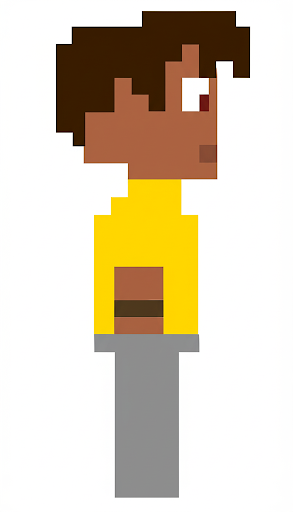
\includegraphics[width=0.5\linewidth]{figs/geminiPro/chat6/tela2_res4.png}
        \legend{\small Fonte: Elaborada pela autora, utilizando a ferramenta Gemini Pro.}
    \end{minipage}\hfill
    \begin{minipage}{0.45\textwidth}
        \centering
        \caption{\small Quadro da animação gerada no Gemini Pro com distorções circuladas em vermelho}
        \label{fig:GeminiProAndarDeformacao}
        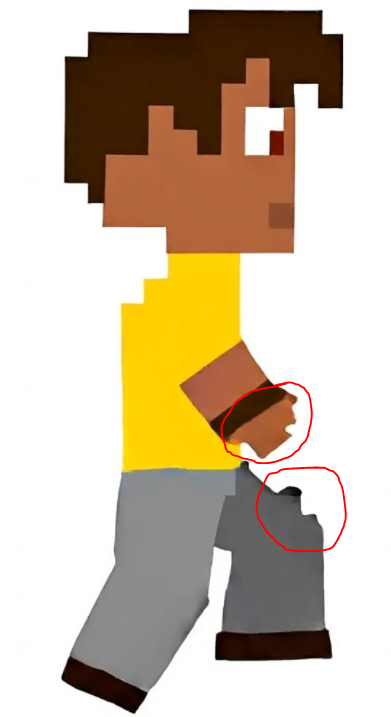
\includegraphics[width=0.5\linewidth]{figs/geminiPro/chat7/deformacoes1.PNG}
        \legend{\small Fonte: Elaborada pela autora, utilizando a ferramenta Gemini Pro.}
    \end{minipage}
\end{figure}

Como foi rapidamente gerada uma animação adequada, os experimentos seguintes focaram em testar se a ferramenta mantém esse alto padrão na geração e se era possível criar um vídeo que não tivesse nenhuma distorção. Para esses testes, uma versão aprimorada do sprite anterior (Figura \ref{fig:GeminiProSideMelhor}) foi utilizada como referência. Os resultados\footnote{\url{https://drive.google.com/drive/folders/19e9IRIDhn1UlBP_wyuXw2AIhyZP0OnSC?usp=sharing}} também foram satisfatórios, apresentando alta consistência e precisão e não possuindo as distorções citadas anteriormente. Porém, ainda foram encontrados pequenos erros de consistência, que podem ser vistos na Figura \ref{fig:GeminiProAndarComparaSpriteSide2}. Apesar disso, um dos vídeos gerados mostrou-se mais adequado do que os prévios, com apenas uma única inconsistência visível (Figura \ref{fig:GeminiProAndarComparaSide2Sprite2}. Os testes completos podem ser consultados nas Figuras \ref{fig:geminiProAndar5} e \ref{fig:geminiProAndar6} no Apêndice \ref{ap.telasIA}. 

\begin{figure}[htbp]
    \centering
    \caption{\small Comparação do sprite de referência com os sprites em side view das animações geradas no Gemini Pro}
    \label{fig:GeminiProAndarComparaSpriteSide2}
    \begin{subfigure}{0.32\linewidth}
        \centering
        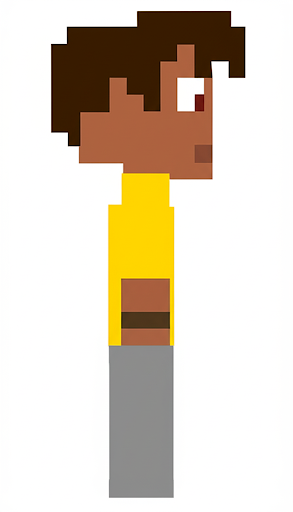
\includegraphics[width=0.7\linewidth]{figs/geminiPro/chat6/tela3_res1.png}
        \caption{\small Sprite do Pablo em side view usado de referência}
        \label{fig:GeminiProAndarSide2}
    \end{subfigure}
    \begin{subfigure}{0.32\linewidth}
        \centering
        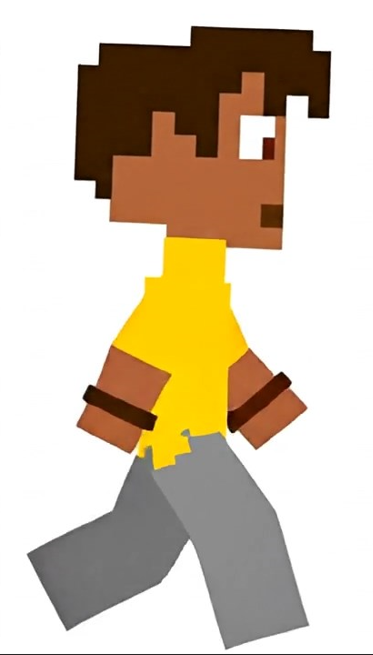
\includegraphics[width=0.7\linewidth]{figs/geminiPro/chat7/sprite2.PNG}
        \caption{\small Sprite com inconsistência na boca e no bracelete}
        \label{fig:GeminiProAndarComparaSide2Sprite1}
    \end{subfigure}
    \begin{subfigure}{0.32\linewidth}
        \centering
        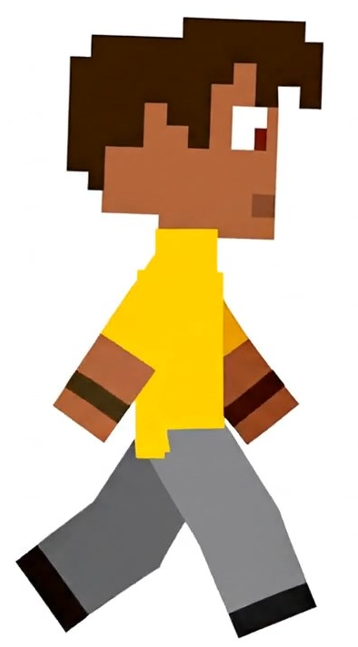
\includegraphics[width=0.7\linewidth]{figs/geminiPro/chat7/sprite3.PNG}
        \caption{\small Sprite com inconsistência no sapato}
        \label{fig:GeminiProAndarComparaSide2Sprite2}
    \end{subfigure}

    \legend{\small Fonte: Elaborada pela autora, utilizando a ferramenta Gemini Pro.}
\end{figure}

 Comparando todos os vídeos gerados, foi possível perceber que as animações geradas usando o personagem em front view como referência apresentavam menos incoerências na pixel art em relação aos que usavam um sprite em side view. Foi levantada a hipótese de que a IA consegue gerar de maneira mais precisa a animação em pixel art quando a referência está no padrão pixel perfect. As imagens em side view não estavam nesse padrão pois tinham sido feitas por IA.

Como havia outras animações para serem geradas, foi decidido fazer a implementação do melhor resultado no jogo. Para isso, o vídeo foi transformado em um sprite sheet (Figura \ref{fig:geminiProAndarSpriteSheet}) usando a ferramenta ezgif (mencionada anteriormente).

\begin{figure}[htbp]
    \centering
    \caption{\small Sprite sheet do vídeo de caminhada gerado no Gemini Pro}
    \label{fig:geminiProAndarSpriteSheet}
    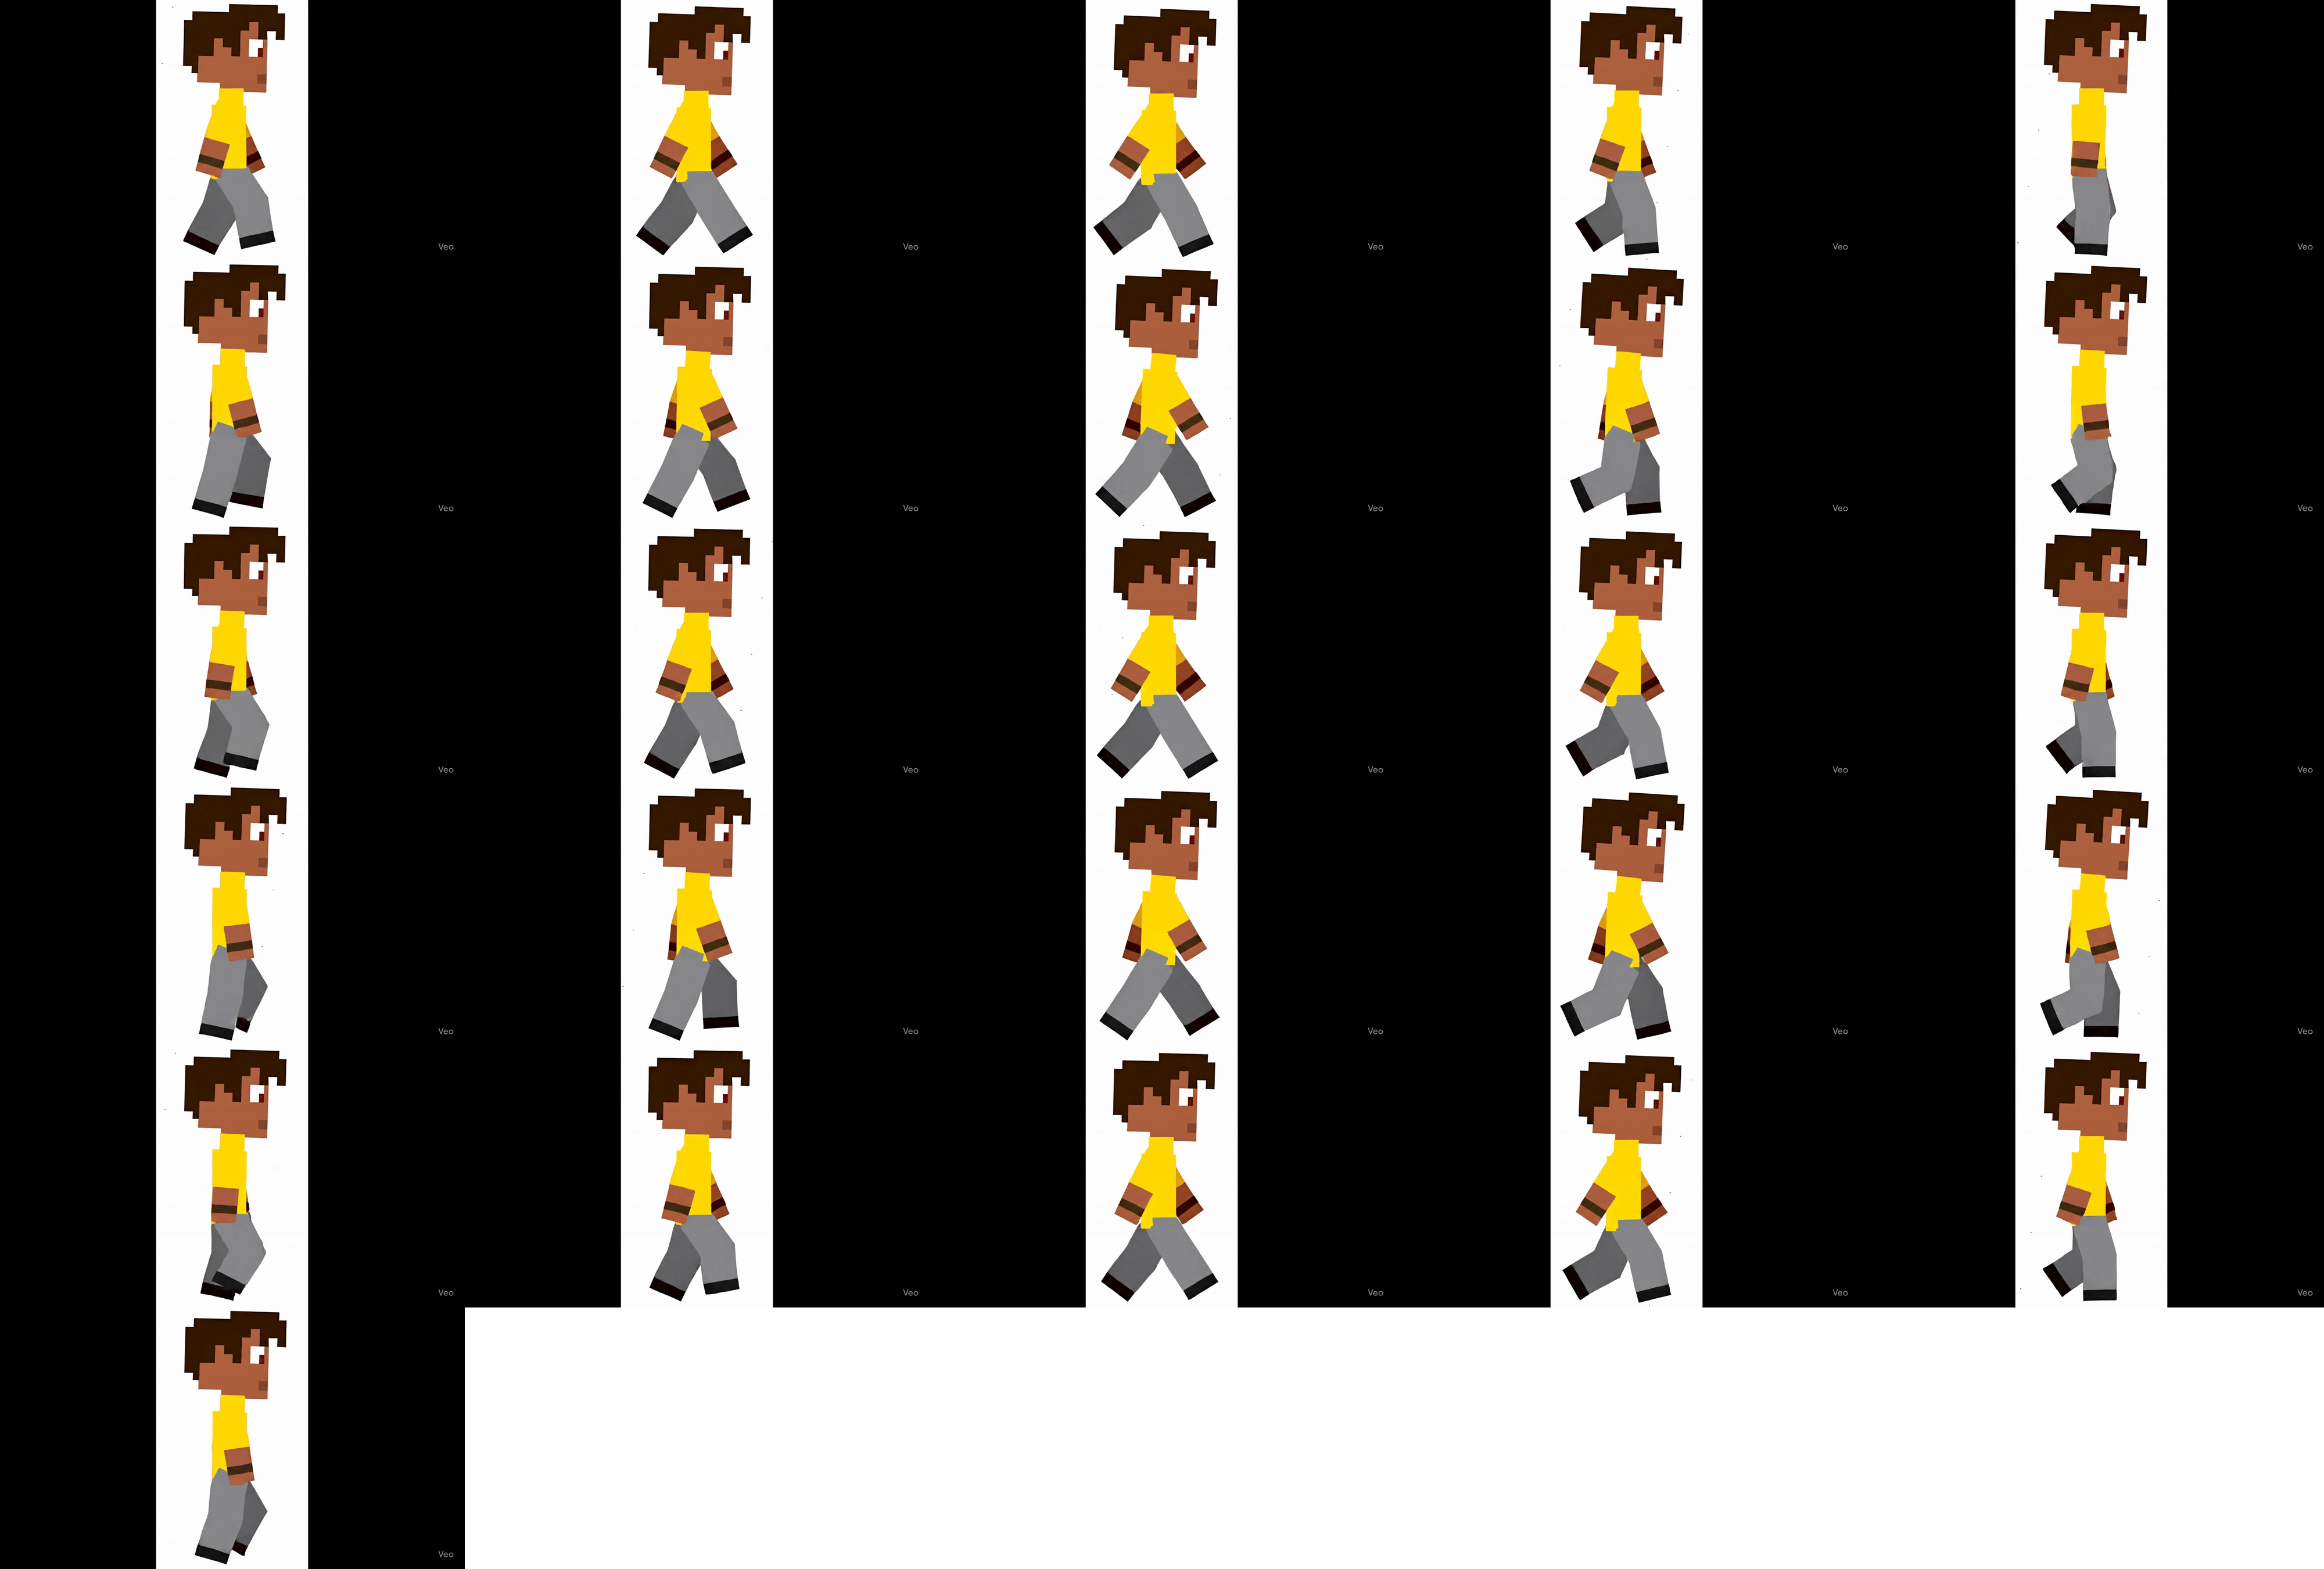
\includegraphics[width=0.8\linewidth]{figs/geminiPro/sprite sheet/video3.png}
    \legend{\small Fonte: Elaborada pela autora, utilizando a ferramenta ezgif.}
\end{figure}

Além disso, também foi necessário remover o fundo da imagem para que o mesmo não aparecesse durante o jogo. Para isso, foi utilizada a ferramenta removebg\footnote{\url{https://www.remove.bg/upload}}. O resultado pode ser consultado na Figura \ref{fig:geminiProAndarSpriteSheetSemFundo}.

\begin{figure}[htbp]
    \centering
    \caption{\small Sprite sheet do ciclo de caminhada sem fundo}
    \label{fig:geminiProAndarSpriteSheetSemFundo}
    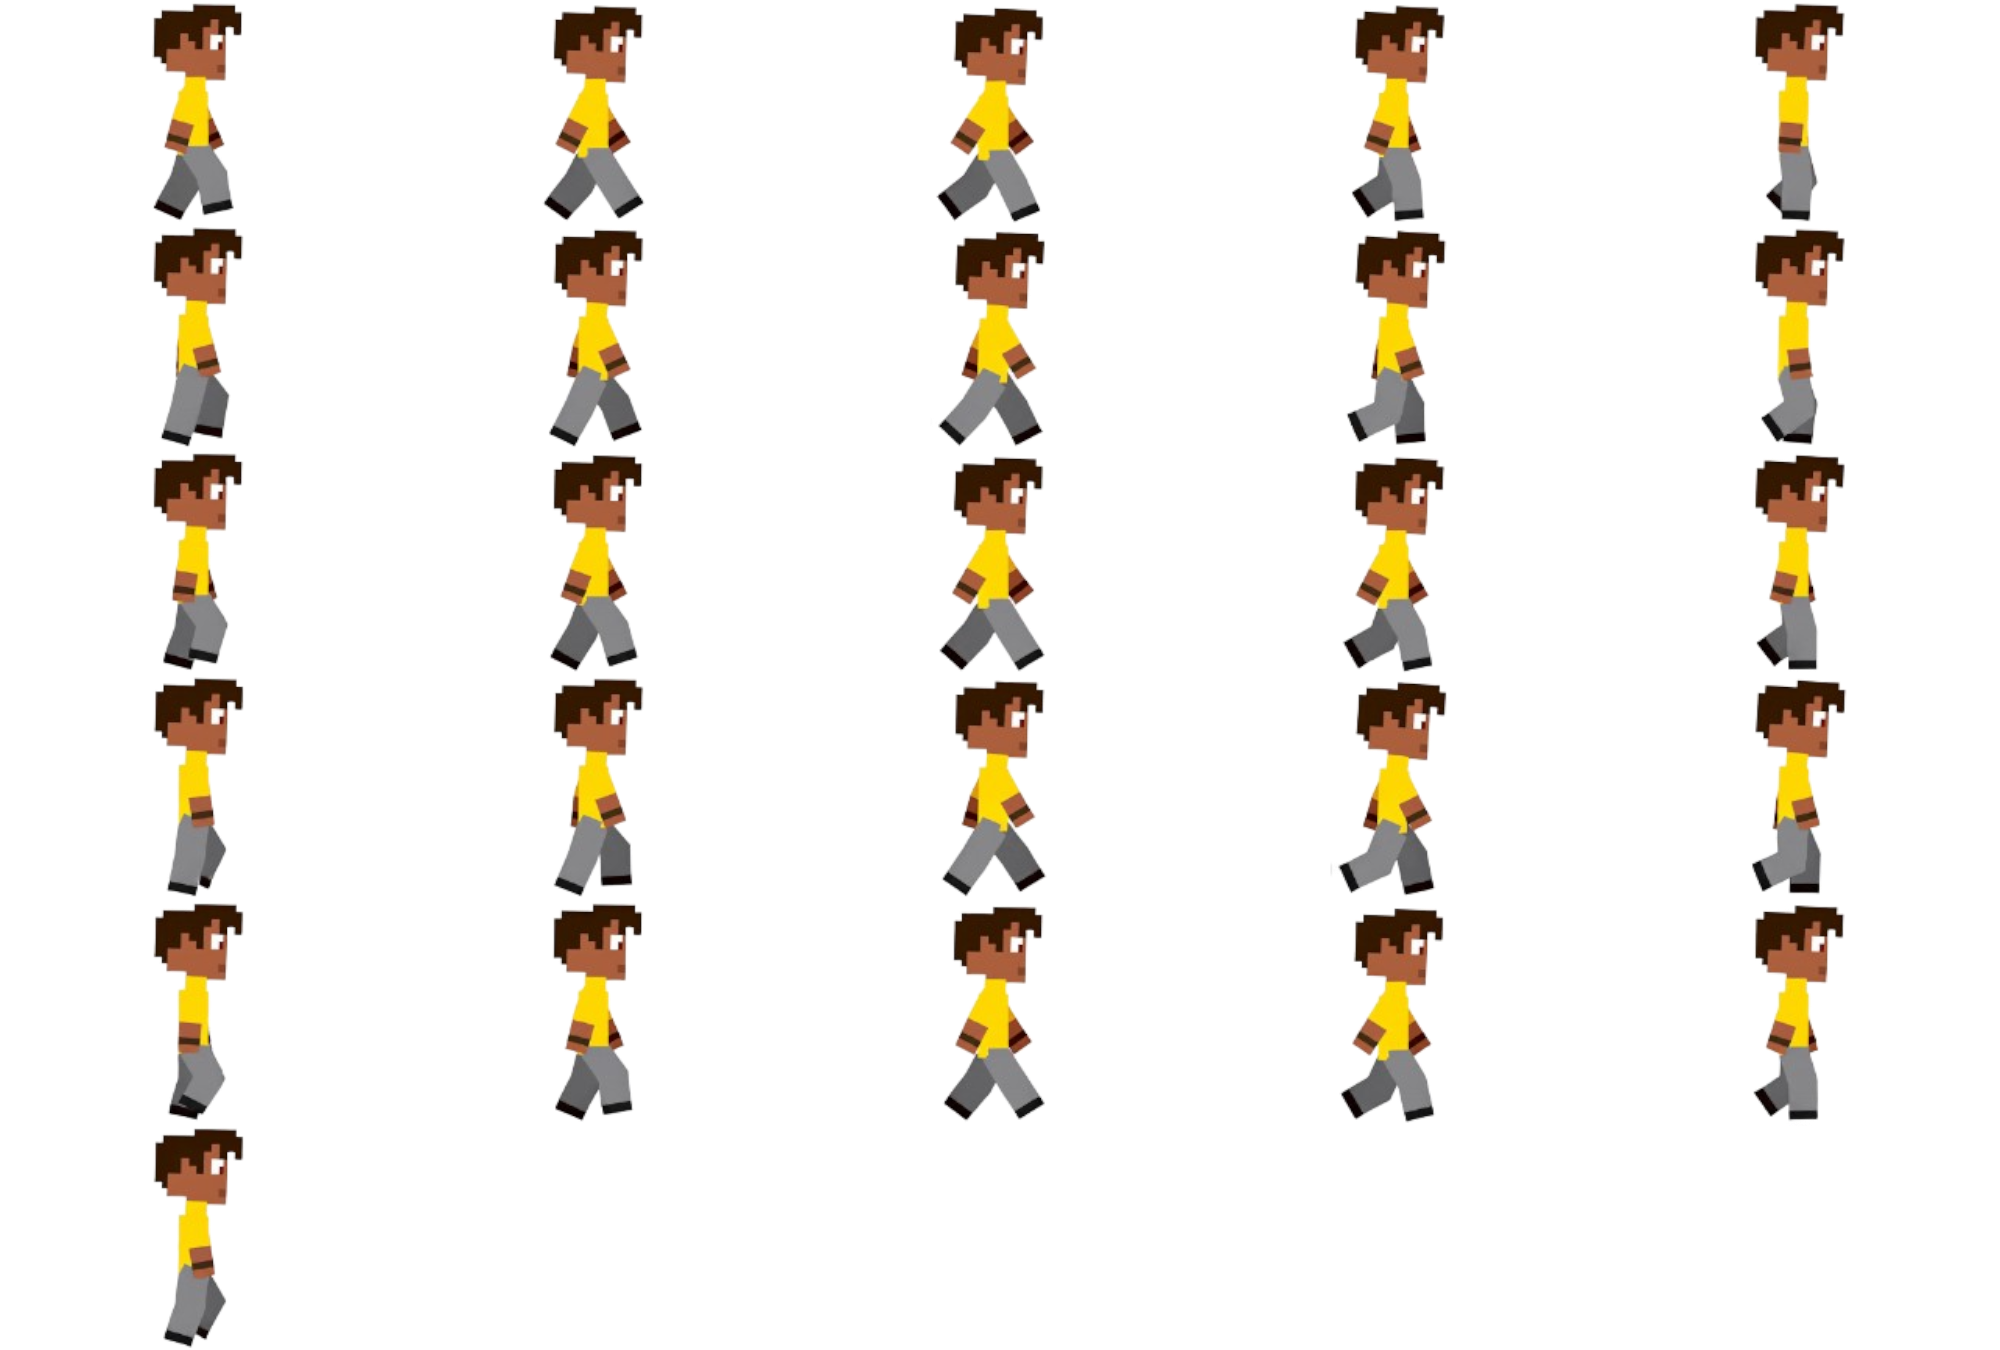
\includegraphics[width=0.8\linewidth]{figs/geminiPro/sprite sheet/sprite_fundo_transparente3.png}
    \legend{\small Fonte: Elaborada pela autora, utilizando a ferramenta removebg.}
\end{figure}



Posteriormente, o sprite em side view foi ajustado e aprimorado no Pixel Lab, o que tornou ultrapassada a imagem usada na animação de caminhada. As diferenças não eram muito grandes, de maneira que o vídeo ainda fosse adequado para ser usado no jogo. Porém, mesmo assim, novos testes foram realizados com a Figura \ref{fig:geminiProPabloPixelLabSide} de referência. Os resultados\footnote{\url{https://drive.google.com/drive/folders/16IjPYloPZtl81zKZ3kOz3I3qkPX078_9?usp=sharing}} não foram melhores do que a animação já implementada, todos apresentando mais erros de consistência que o anterior, em específico fazendo o bracelete ganhar um relevo que dava uma vaga sensação de 3D, como pode ser visto na Figura \ref{fig:GeminiProAndarBracelete3D}. Diversos prompts diferentes foram usados em busca de corrigir essa falha, porém não houve sucesso. Também é importante notar que alguns dos resultados conseguiram parcialmente manter a coerência da pixel art durante a animação (Figura \ref{fig:GeminiProAndarCoerencia}). Isso consolida a hipótese levantada antes sobre a IA ter mais facilidade em animar de maneira pixelada ao se usar um sprite no padrão pixel perfect, como foi o caso durante esses testes. Todas as interações podem ser consultadas nas Figuras \ref{fig:geminiProAndar7} a \ref{fig:geminiProAndar12} no Apêndice \ref{ap.telasIA}.

\begin{figure}[htbp]
    \centering
    \begin{minipage}{0.45\textwidth}
        \centering
        \caption{\small Sprite com o bracelete 3D na animação de caminhada gerado no Gemini Pro}
        \label{fig:GeminiProAndarBracelete3D}
        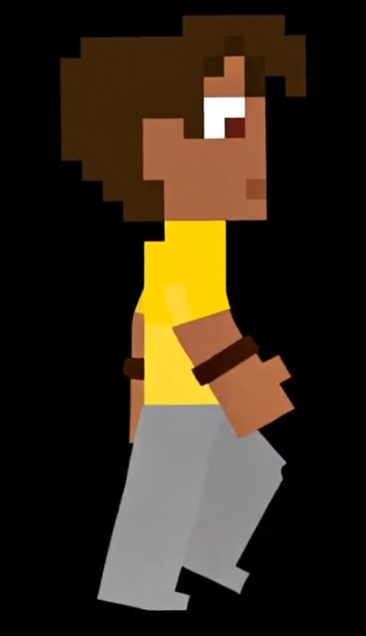
\includegraphics[width=1\linewidth]{figs/geminiPro/chat7/bracelete3D.PNG}
        \legend{\small Fonte: Elaborada pela autora, utilizando a ferramenta Gemini Pro.}
    \end{minipage}\hfill
    \begin{minipage}{0.45\textwidth}
        \centering
        \caption{\small Quadro da animação parcialmente coerente com o estilo pixel art gerada no Gemini Pro}
        \label{fig:GeminiProAndarCoerencia}
        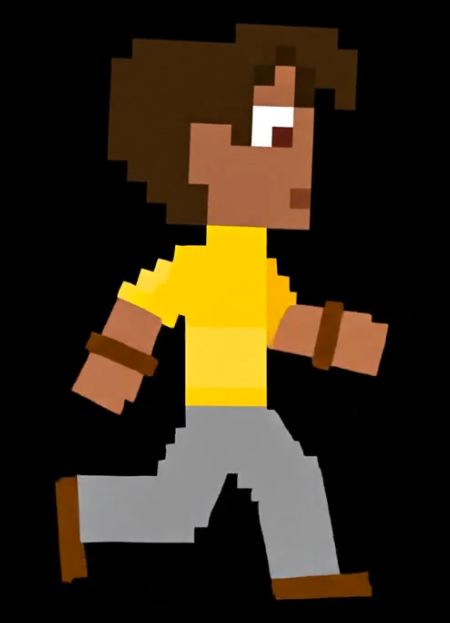
\includegraphics[width=1\linewidth]{figs/geminiPro/chat7/animacaoParcialmenteCoerente.PNG}
        \legend{\small Fonte: Elaborada pela autora, utilizando a ferramenta Gemini Pro.}
    \end{minipage}
\end{figure}

De maneira não planejada, uma animação de caminhada satisfatória com o sprite final foi obtida durante os experimentos de gerar a animação do personagem abrindo a porta, conforme será detalhado na Seção \ref{s.gemini.animacaoAbrir}.

A ferramenta Gemini Pro demonstrou uma alta capacidade de precisão e consistência para a geração de animações 2D, sendo parcialmente capaz de lidar com o estilo de pixel art. Algumas pequenas distorções e inconsistências podem ser encontradas nos vídeos, porém são detalhes pouco significativos que podem ser corrigidos através de um ajuste manual, trazendo um ganho de tempo em comparação a desenhar o personagem do zero para cada frame. Esse processo de edição, entretanto, se torna mais complicado pelo fato de que a ferramenta não apresenta um editor embutido.

